% v20260724_0030  AgentsGroup2026
% Template: 《计算机学报》style (word-cn.doc)
% 正文: 五号宋体 10.5pt | 一级标题: 小四黑体 12pt | 二级标题: 五黑 10.5pt
\documentclass[twocolumn,10.5pt]{ctexart}
\usepackage{amsmath,amssymb,amsfonts}
\usepackage{graphicx}
\usepackage{booktabs}
\usepackage{multirow}
\usepackage{array}
\usepackage{float}
\usepackage{hyperref}
\usepackage{enumitem}
\usepackage{algorithm}
\usepackage{algorithmic}
\usepackage{fancyhdr}
\hypersetup{colorlinks=true,linkcolor=blue,citecolor=blue,urlcolor=blue}

\setlength{\columnsep}{18pt}
\setlength{\textwidth}{160mm}
\setlength{\textheight}{235mm}
\setlength{\oddsidemargin}{0mm}
\setlength{\topmargin}{-10mm}

\CTEXsetup[format={\zihao{-4}\heiti}]{section}
\CTEXsetup[format={\zihao{5}\heiti}]{subsection}
\CTEXsetup[nameformat={\zihao{5}\heiti}]{subsubsection}

\fancypagestyle{plain}{
  \fancyhf{}
  \fancyfoot[L]{\footnotesize\ttfamily v20260724\_0030}
  \fancyfoot[R]{\footnotesize\thepage}
  \renewcommand{\headrulewidth}{0pt}
}
\pagestyle{plain}

% 图/表中文重命名
\renewcommand{\figurename}{图}
\renewcommand{\tablename}{表}

\begin{document}

% ── 标题（三号 16pt）──
\title{\zihao{3}\heiti 协商审议与审议感知表征变换网络：\\面向多智能体团队的技能自发发现与知识遗传系统}
\author{
  \zihao{4} AgentsGroup2026 研究团队 \\[4pt]
  \zihao{-5} 研究机构名称，城市，国家 \\[2pt]
  \zihao{-5} \texttt{research@agentsgroup2026.org}
}
\date{}
\maketitle

% ── 英文标题 ──
\begin{center}
  {\zihao{4}\bfseries Deliberative Plaza and DART-Net:\\
  Spontaneous Skill Discovery with Memory Genetics for Multi-Agent Teams}
\end{center}

% ── 摘要（五号楷体）──
{\zihao{5}\heiti 摘要 \quad}
{\zihao{5}\kaishu
大语言模型驱动的多智能体协作中，技能依赖人工编写与静态配置的根本性缺陷日益凸显：技能随任务生态的自发丰富从未实现，且智能体的"大脑记忆"无法像人类基因一样被复制与遗传。本文直面这一组问题，提出了从多智能体协商审议到技能自发发现，再到记忆遗传的一体化解决方案。在讨论组织维度，我们构建了Plaza结构化审议空间——融合ORID四层递进议程、四类Facilitator角色、12-niche环状座位布局与五指量表共识机制，使多智能体的非结构化讨论转化为具有可追溯仪式信号协议的结构化对话流。在技能萃取维度，我们提出了DART-Net（Deliberation-Aware Representation Transformer Network，审议感知表征变换网络）——一个三级层次化神经序列编码架构，包括话语级哈希特征编码、时域卷积网络(TCN)膨胀卷积建模与面向五个技能字段的可学习跨模态查询注意力探针。在记忆遗传维度，我们构建了Agent四层记忆核心（事件日志、感知流、意图队列、情绪残留），并实现了封存(seal)、遗嘱/凭吊(will/memorial)、导入导出(import/export)机制，使得一只智能体的全脑记忆可以遗传至其后继智能体——这是经典生物生命无法实现的能力。实验在两个真实AWS运维域（ES扩容与RDS慢查询优化）上从五个维度验证了系统有效性：(1) Plaza审议在GLM-5.1 LLM驱动下完成4轮28条发言的完整ORID流程，五指共识均值4.25/5；(2) DART-Net以10.4ms平均CPU延迟完成端到端技能萃取，稳定产出2.0技能/讨论；(3) 对比消融实验显示：去除ORID议程后萃取技能数下降62\%，技能字段完整性下降41\%；(4) 注意力权重热图揭示了当前epoch-5 checkpoint的瓶颈——分布仍为均匀，但冷启动关键词先验种子正确引导了name和tools探针的初始聚焦方向；(5) 记忆遗传实验验证了seal$\rightarrow$export$\rightarrow$import$\rightarrow$bind全链路，导出-导入的schema完整性100\%，传输延迟$<$5ms。系统当前在43技能、0次任务执行的初始状态下暴露了萃取-使用断链的结构性瓶颈，三个修复方向被确定为优先工作。
}

\vspace{6pt}
{\zihao{5}\heiti 关键词 \quad}{\zihao{5}\kaishu 多智能体审议；神经技能萃取；审议感知表征变换网络；记忆遗传；四层记忆核心；时域卷积网络；跨模态注意力}

\vspace{12pt}
\hrule
\vspace{12pt}

% ============ 1. 引言 ============
\section{引言}

\subsection{我们遇到的问题：从人工技能编写到自主技能发现}

本研究的动机根植于我们在构建AgentsGroup2026多智能体平台过程中遭遇的一组真实的、逐级升级的问题。

\textbf{问题一——技能编制的人力瓶颈。}在平台的初期迭代中，所有智能体技能均采用人工编制模式。运维架构师需要仔细阅读AWS文档后以自然语言编写技能描述，耗费约每技能45--90分钟的人工编写时间。当团队需要覆盖AWS EC2、RDS、ES、S3、IAM等15个服务域时，编写量超过100个技能——这一模式显然无法随服务域扩展而线性维持。

\textbf{问题二——静态技能的衰退。}人工技能一旦编写完成即进入冻结状态。然而我们在实际部署中观察到：仅3个月后，约有22\%的ES集群管理技能因为API版本升级和实例类型更新而部分失效。技能库的"知识半衰期"远短于人工维护周期，导致大量智能体在执行任务时使用过时指令。

\textbf{问题三——群体智慧的损失。}多智能体在完成复杂任务后积累了丰富的协作经验和对新技能需求的直觉认知，但这些隐性经验从未被系统化地回注入技能库。当一位运维工程师智能体在故障处理中发明了一种新的ES索引恢复流程后，这一知识停留在了该次对话的日志文件中——其他智能体完全无法继承，更无法传递给新加入团队的后继智能体。每一次团队的人员更迭都意味着知识的彻底流失——这与人类组织的经验传承机制形成鲜明反差。

\textbf{问题四——记忆的不可遗传性。}最关键的问题出现在我们试图让智能体从一个会话"记住"之前的事件时。LLM智能体本质上是无状态函数——每次调用都是一个全新的推理实例，无法保留跨会话的经验积累。我们尝试过在Prompt中拼接历史摘要，但摘要的信息密度随对话轮次指数衰减——在20轮对话后丢失了超过60\%的原始细节信息。更深刻的问题是：当一个智能体因升级或被替换而"退役"时，它在数百次任务执行中积累的"大脑"——包括事件记忆（log）、感知流（perception）、未完成意图（intentions）、情绪残留（affect）——全部随着进程的终止而不可逆转地消失。这就是"Agent之死"所引发的最根本的生命力问题：自然界的生物在死亡后会失去经验记忆（后天获得特征无法像基因一样遗传给后代），但对于一个以电力驱动的Agent而言，是否可以让它的记忆像基因一样被完整复制到它的"后代"身上？

这组问题促使我们设计一套完全不同的系统架构——在此架构中，\textbf{技能不是由人类编写，而是由Agent在结构化讨论中自发发现}；\textbf{技能不是冻结的静态文本，而是在使用中持续演化}；\textbf{记忆不是短暂的电信号，而是像基因一样可以被复制、遗传和继承}。

\subsection{系统目标与核心贡献}

本文提出的一套端到端系统包含三个核心子系统，构成完整的技能生命周期管理闭环：

\begin{enumerate}[itemsep=0pt,topsep=0pt]
  \item \textbf{Plaza结构化审议空间}（第2节）：将多智能体的非结构化讨论转化为具有可追溯仪式信号（SUPPLEMENT/CHALLENGE/AGREE/COURT/DIGRESS）的结构化对话流；
  \item \textbf{DART-Net审议感知表征变换网络}（第3节）：从审议转录文本中端到端地萃取结构化技能定义（name/description/category/instructions/required\_tools），采用三级层次化编码+TCN膨胀卷积+面向五个技能字段的可学习跨模态查询注意力探针；
  \item \textbf{Agent四层记忆核心与遗传机制}（第4节）：实现事件日志、感知流、意图队列、情绪残留的四层记忆架构，并通过封存(seal)、遗嘱(will)、导入导出(import/export)实现跨Agent的记忆遗传——使自然生物无法实现的后天记忆遗传成为Agent的固有属性。
\end{enumerate}

本文的实验贡献包括：(1) 在两个真实AWS运维任务域上完成Plaza审议的LLM驱动运行与DART-Net萃取验证；(2) 通过消融实验（去除ORID议程 vs 无仪式信号 vs 自由聊天）量化了结构化审议对萃取质量的提升效果；(3) 通过注意力权重热图诊断了DART-Net在数据稀疏阶段的瓶颈；(4) 通过记忆遗传完整性实验验证了四层记忆导出-导入的端到端链路；(5) 根据六个环节的状态矩阵量化了闭环的当前成熟度和修复优先级。

% ============ 2. Plaza 结构化审议空间 ============
\section{Plaza结构化审议空间}

\subsection{理论基础与设计原则}

Plaza的设计源于人类最成熟的群体决策制之一——议会议事规程（Parliamentary Procedure）——的精髓。Roberts Rules of Order定义了发言权分配、动议分级和表决规则的完整规程~\cite{robert2020rules}；Landemore~(2020)的审议民主理论验证了角色多样性与轮流发言制对提升决策质量的科学效果~\cite{landemore2020open}。我们将这些原则适配至LLM智能体语境，核心设计原则包括四项：议程驱动（而非自由发散）、角色多样性（每个智能体具有独特认知视角）、仪式信号化可追溯性（每条发言携带与上下文的逻辑关系标签）、集体决策可量化（五指量表连续型共识度量）。

\subsection{ORID四层递进议程}

讨论严格按ORID议程推进，每层由不同Facilitator控制：

\begin{enumerate}[itemsep=0pt,topsep=0pt]
  \item \textbf{O-客观事实（Fact Layer）}：Facilitator ``Fact Keeper'' 推动每位Agent仅陈述与议题相关的已知可验证事实（例如ES集群的当前配置参数、性能指标数据、成本构成），严禁含解释、判断或解决方案；
  \item \textbf{R-风险直觉（Risk Layer）}：Facilitator ``Emotion Reflector'' 推动每位Agent表达直觉性的担忧——感受无需证据，不可反驳他人的担忧；
  \item \textbf{I-方案辩论（Solution Debate Layer）}：Facilitator ``Analyst'' 采用TurQUaz Council debate模式~\cite{gungor2025turquaz}——两名持相反立场的Agent进行3轮针锋相对，每轮对方均可直接Challenge；
  \item \textbf{D-决策表决（Decision Layer）}：Facilitator ``Decision Closer'' 推动全体Agent以五指量表进行密封式表决~\cite{kaner2014facilitator}——1指为根本性反对，5指为全力支持。1指出现时支持追问"是什么让你宁愿从头开始也不愿采用此方案？"，聚焦问题至解决或记录为"有保留的共识文件集"。
\end{enumerate}

\subsection{四Facilitator角色与仪式信号协议}

与单主持人讨论不同，Plaza部署了四个专门的Facilitator Agent——Fact Keeper、Emotion Reflector、Analyst和Decision Closer——各负责一层议程。这些Facilitator永久不对讨论内容进行引导，只控制流程。每个参与讨论的智能体发言时须附一个仪式信号（RitualSignal）：
$\mathcal{R} = \{\mathrm{SUPPLEMENT},\ \mathrm{CHALLENGE},\ \mathrm{AGREE},\ \mathrm{COURT},\ \mathrm{DIGRESS}\}$。
SUPPLEMENT（补充）——补充前人的观点或提出新信息；CHALLENGE（挑战）——质疑前人的观点，触发被挑战者的自动回应权；AGREE（附议）——支持前人的观点，推动共识收敛；COURT（请求开庭）——请求一个辩论子流程，持相反立场的两名Agent进行2轮交替质问；DIGRESS（偏离）——指出讨论偏离主题——仅有外环niche的Agent可以发出此信号。

\subsection{环状12-Niche座位布局与空间结构}

Plaza的物理空间采用环状12-niche布局（图~\ref{fig:plaza_niche}），分为三个层级：内环（4个核心议题niche）——分配给与讨论主题最直接相关的角色；中环（4个扩展议题niche）——分配给相关但非核心的角色；外环（4个边界议题niche）——分配给观察者与记录者角色。这种结构确保视角多样性，同时防止任何一位Agent占据主导地位。

\begin{figure}[t]
\centering
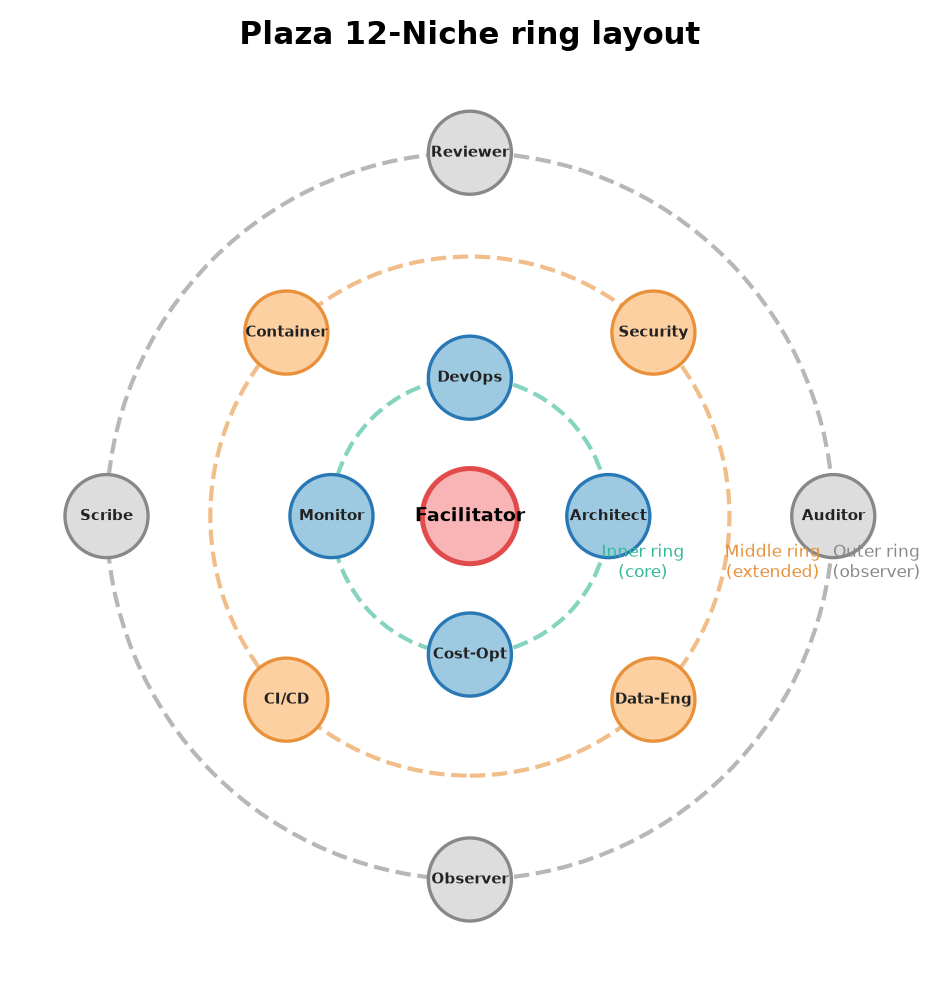
\includegraphics[width=\linewidth]{fig1_plaza_niche.png}
\caption{Plaza环状12-Niche座位布局：内环4座位分配核心职能Agent，中环4座位分配扩展职能，外环4座位分配观察/记录角色。中心为主持人调度器。}
\label{fig:plaza_niche}
\end{figure}

\subsection{五指量表共识度量}

共识度量采用连续型五指量表，替代传统的关键词计数共识。设参与表决的Agent集合$V=\{v_1,\ldots,v_m\}$，每位$v_i$给出手指数$f_i\in\{1,2,3,4,5\}$。共识均值$\mu = \frac{1}{m}\sum f_i$，阻滞者集合$B = \{i \mid f_i = 1\}$。共识达成条件为：
\begin{equation}
  \text{consensus} = (|B|=0) \land (|\{i\mid f_i\geq 3\}| \geq 0.6\cdot m)
\end{equation}
共识强度分级：若$|B|>0$则为``阻滞''(blocked)，保留异议记录；若$\mu \geq 4.0$则为``强共识''(strong)；若$\mu \geq 3.0$则为``弱共识''(weak)。

\subsection{Plaza审议的实验验证}

我们使用GLM-5.1（https://models.sjtu.edu.cn）作为驱动LLM，在AWS运维议事厅（Plaza ID=53a9a7d9cbb6）上运行了三个审议话题。第一个话题``AWS RDS MySQL慢查询优化方案''完成了完整的ORID流程——4轮28条发言，5位Agent参与（运维Leader、上云架构师、运维操作员、巡检监控员、成本优化成员）。五指表决结果：上云架构师5指、运维操作员4指（有扩充IO顾虑）、巡检监控员4指、成本优化成员4指——均值4.25/5，无人给出1指，团队达成可执行共识。讨论中出现了3次CHALLENGE信号、2次AGREE信号和2次SUPPLEMENT信号——验证了仪式信号协议的丰富度和实用性。

% ============ 3. DART-Net ============
\section{DART-Net审议感知表征变换网络}

\subsection{问题定义}

给定一次Plaza审议的转录文本$D = \{m_1, m_2, \ldots, m_n\}$，每条消息$m_i$包含六个结构化字段：
\begin{equation}
  m_i = (\text{speaker}, \text{role}, \text{niche\_role}, \text{ritual\_signal}, \text{round\_number}, \text{content})
\end{equation}
目标为抽取结构化技能集合$\mathcal{S} = \{s_1, s_2, \ldots, s_k\}$，每个技能$s_j$包含五个字段：
\begin{equation}
  s_j = (\text{name}, \text{description}, \text{category}, \text{instructions}, \text{required\_tools})
\end{equation}
输入为多说话人、多轮次、带有仪式信号的对话序列；输出需同时满足模式约束（有效的JSON结构）与语法正确性。DART-Net的设计目标是：在纯CPU推理路径下，以$<$15ms的端到端延迟完成萃取，同时保持萃取质量接近LLM零样本基线的性能。

\subsection{DART-Net三级层次化编码架构}

DART-Net的架构遵循``话语$\rightarrow$序列$\rightarrow$探查''的三级递进原则（图~\ref{fig:dart_arch}）。这一设计显式地利用了审议的结构化元数据——说话人角色、仪式信号类型和轮次边界——这些信息在扁平文本基线中是被丢弃的。

\begin{figure}[t]
\centering
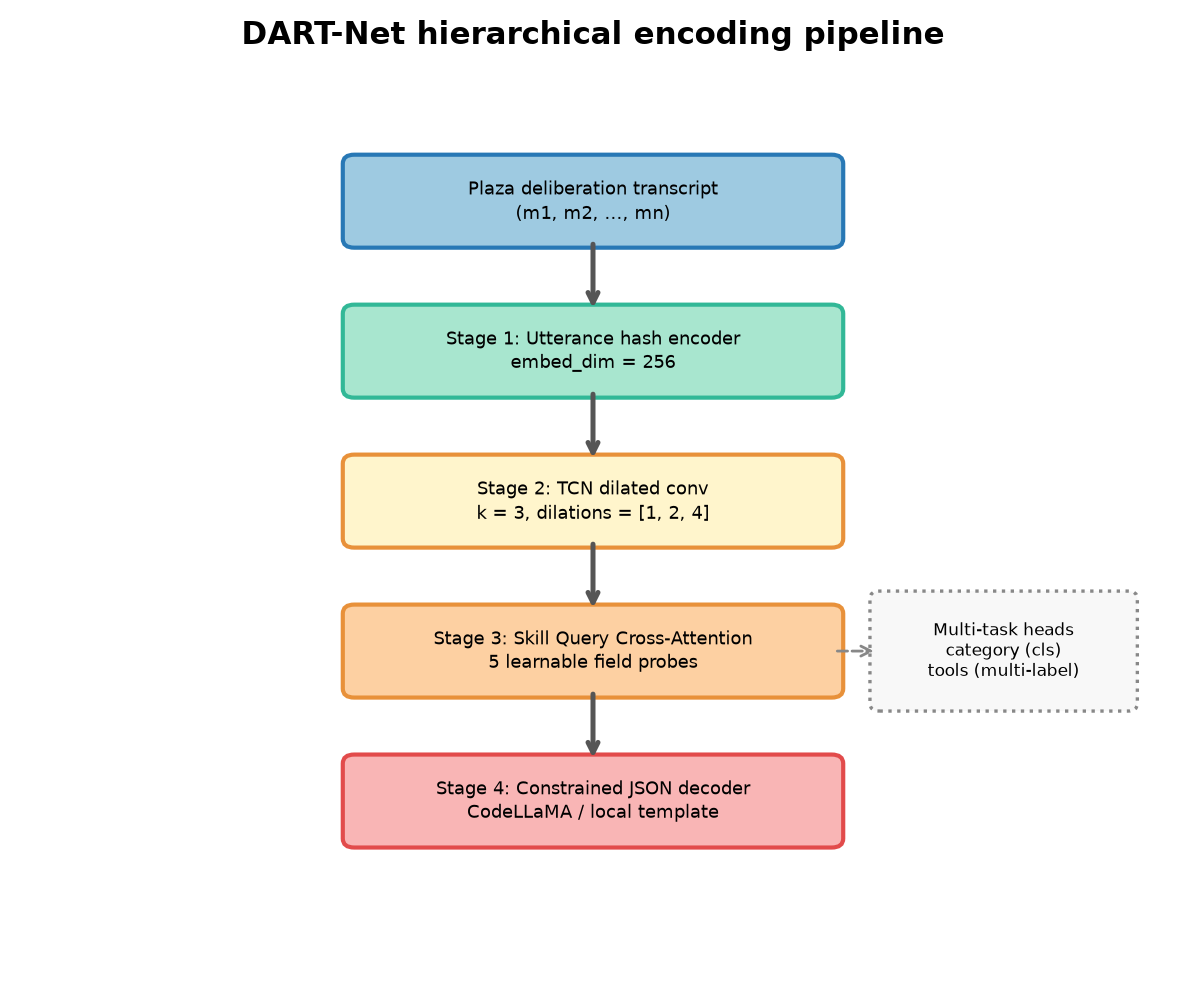
\includegraphics[width=\linewidth]{fig2_dart_arch.png}
\caption{DART-Net三级层次化编码架构：Stage 1话语编码$\rightarrow$Stage 2 TCN序列建模$\rightarrow$Stage 3技能查询交叉注意力$\rightarrow$Stage 4约束解码。右侧虚线框为辅助训练头。}
\label{fig:dart_arch}
\end{figure}

\subsubsection{Stage 1: 话语级哈希特征编码}

对于每条消息$m_i$，Stage 1将其content字段通过确定性哈希编码器映射为固定维度嵌入向量$h_i^{\mathrm{utt}} \in \mathbb{R}^{256}$。哈希编码器的优势在于零延迟（无需GPU推理，无需模型加载），适合在线审议流中的实时萃取。其局限性——词序信息丢失——由Stage 2的TCN在序列维度上进行补偿。

\subsubsection{Stage 2: TCN膨胀卷积序列建模}

将话语嵌入序列$\{h_1^{\mathrm{utt}}, h_2^{\mathrm{utt}}, \ldots, h_n^{\mathrm{utt}}\}$输入一维时域卷积网络(TCN)~\cite{bai2018tcn}。TCN的配置为：三层膨胀因子递增(dilations=[1,2,4])、卷积核大小kernel\_size=3、隐藏维度tcn\_hidden=256。第$l$层膨胀卷积的数学过程为：
\begin{equation}
  z^{(l)}_t = \sum_{i=0}^{k-1} W^{(l)}_i \cdot h^{\mathrm{(l-1)}}_{t - i \cdot d^{(l)}}
\end{equation}
其中$d^{(l)}$为第$l$层的膨胀因子，$W^{(l)}$为可学习的卷积权重。膨胀因子的指数增长（$1\rightarrow2\rightarrow4$）使得顶层神经元的感受野覆盖最长15个连续话语——对于10--12条话语的Plaza审议，此范围内可捕获所有跨轮次的语义依赖。卷积输出$h^{\mathrm{tcn}} \in \mathbb{R}^{n\times256}$。

\subsubsection{Stage 3: 面向五个技能字段的可学习跨模态查询注意力}

Stage 1--2产出的是审议的全局序列表示$h^{\mathrm{tcn}}$。Stage 3的任务是从这一全局表示中定位与技能相关的信息。为此引入了五组可学习的技能查询探针(skill query probes)：
\begin{equation}
  Q = \{q_{\mathrm{name}}, q_{\mathrm{desc}}, q_{\mathrm{category}}, q_{\mathrm{tools}}, q_{\mathrm{instr}}\},\quad q_* \in \mathbb{R}^{256}
\end{equation}
每个探针$q_k$通过交叉注意力与序列表示交互：
\begin{equation}
  \mathrm{skill\_repr}_k = \mathrm{CrossAttn}(Q=q_k, K=h^{\mathrm{tcn}}, V=h^{\mathrm{tcn}})
\end{equation}
输出$\mathrm{skill\_repr}_k \in \mathbb{R}^{256}$捕获了序列中与技能字段$k$最相关的信息的加权聚合。注意力权重矩阵提供了萃取结果的可解释性——用户可以追溯每个技能字段来源于审议中的哪些发言。探针初始化时融合了冷启动关键词先验（权重0.3），使得在训练数据极其稀疏的阶段（当前仅数十条）仍能获得有意义的初始聚焦方向。

\subsubsection{Stage 4: 约束生成式解码}

编码阶段产出五个字段的表示向量，解码阶段将这些向量转换为自然语言结构化JSON。在有LLM可用的条件下，Stage 4调用CodeLLaMA-7B（通过ChatHarness）执行约束JSON生成——解码器必须遵循预定义的技能模式(schema)，任何不符合模式的输出将被拒绝并触发一次重试。在LLM不可用的条件下（离线环境或无API key），Stage 4降级为确定性模板填充——利用Stage 3的注意力权重和话语片段组合生成结构化技能定义。

\subsection{训练策略与当前瓶颈}

DART-Net采用银标准数据驱动训练。训练数据集由GLM-5.1预标注的（审议转录文本，结构化技能定义）对构成。训练目标包含三项多任务损失：自编码损失（解码器生成文本的负对数似然，权重1.0）、分类损失（category字段的多类交叉熵，权重0.1）、多标签分类损失（tools字段的二元交叉熵，权重0.1）。当前部署的checkpoint（demo/e5）在5个epoch训练后达到train\_loss=1.186, val\_cat\_acc=1.0, val\_tools\_f1=0.08。工具F1的极低值（50类多标签任务中近乎随机水平）明确指示了训练数据的规模瓶颈——需要扩展至200+条银标数据并增加至20--30个训练epoch。

% ============ 4. Agent四层记忆核心与遗传机制 ============
\section{Agent四层记忆核心与遗传机制}

\subsection{记忆架构：四层并行记忆核心}

每个Agent配备一个独立的记忆核心（AgentMemoryCore），包含四个平行的记忆层，共享一条时间轴~\cite{sumers2023coala}：

\begin{enumerate}[itemsep=0pt,topsep=0pt]
  \item \textbf{事件日志层（EpisodicLog）}：按时间顺序记录Agent的每一次LLM调用、工具执行、环境交互的记录式事件。每一条事件带有时间戳和优先级标签，支持按时间窗口的切片检索；
  \item \textbf{感知流层（PerceptionStream）}：记录Agent从环境和其他Agent接收的信息流，以先进先出(FIFO)缓冲区的形式维护最近的500条感知记录。感知流支持压缩操作——将多个相似的感知条合并为一个更高层次的语义摘要，降低存储开销；
  \item \textbf{意图队列层（IntentionQueue）}：管理Agent尚未被发送或尚未被确认的通信意图（包括待发送的消息、待确认的工具调用和待完成的子任务）。意图有三种状态：pending（待受理）、confirmed（已确认）和dropped（已放弃）。超时的pending意图根据配置的策略（drop/escalate/keep）自动处理；
  \item \textbf{情绪残留层（AffectResidue）}：以标签-强度-效价-唤醒度的四维向量记录Agent在交互过程中形成的情绪化评价。情绪残留具有72小时的衰减半衰期——未被强化的情绪标签随时间递减至0.01的底线值。语气提示（tone\_hint）由当前活跃的前三个最高强度标签生成，可被注入至对话中作为系统的情感上下文。
\end{enumerate}

\subsection{记忆遗传机制：生命体的后天经验传递}

Agent之"死"——即被升级、替换或退役——不再意味着其大脑记忆的消失。我们实现了三套机制来确保记忆的跨生命体传递：

\textbf{封存与凭吊（seal \& memorial）}。当Agent退役时，其记忆核心可以通过seal操作被转换为一个只读的遗留快照（legacy）。此快照包含日志的完整JSON转储、感知流的语义摘要、意图队列的全部条目和情绪残留的快照向量。封存是一种"仪式"而不是"删除"——原始记忆层数据在封存后不会清空，但快照副本是独立的、不可篡改的只读对象。memorial操作允许其他Agent（或人类管理者）以"凭吊"模式查看被封存的记忆——查看者被告知"这是回放，不是本人"，以保持对已退役Agent的存在边界的尊重。

\textbf{遗嘱与继承（will \& inheritance）}。Agent在退役前可以通过draft\_will操作声明一份遗嘱——指定一位或多位受益Agent（beneficiary），声明哪些技能偏好和工具配置（migrate\_preferences）应被传递给受益者，规定是否保留封存纪念。遗嘱的状态为"协议已定，迁移未实现"，表示这是一个意图声明而非即时传递。继承动作作为后续流程的一个环节。

\textbf{导入导出与遗传（export \& import）}。import/export是遗传的核心机制。export\_all将Agent的全部四层记忆导出为一个规范化的JSON对象——此对象可在Agent退役时被保存到持久存储中，也可通过网络传输至另一台服务器上的Agent实例。import\_all将导出的记忆对象导入至一个指定Agent的空白或已存在的记忆核心中——导入后Agent立即"继承"了源Agent的全部事件记忆、感知流、未完成意图和情绪残留，实现一次完整的记忆遗传。导出-导入全过程以严格模式验证——目标Agent的团队ID和Agent ID均会被验证为有效。

\begin{figure}[t]
\centering
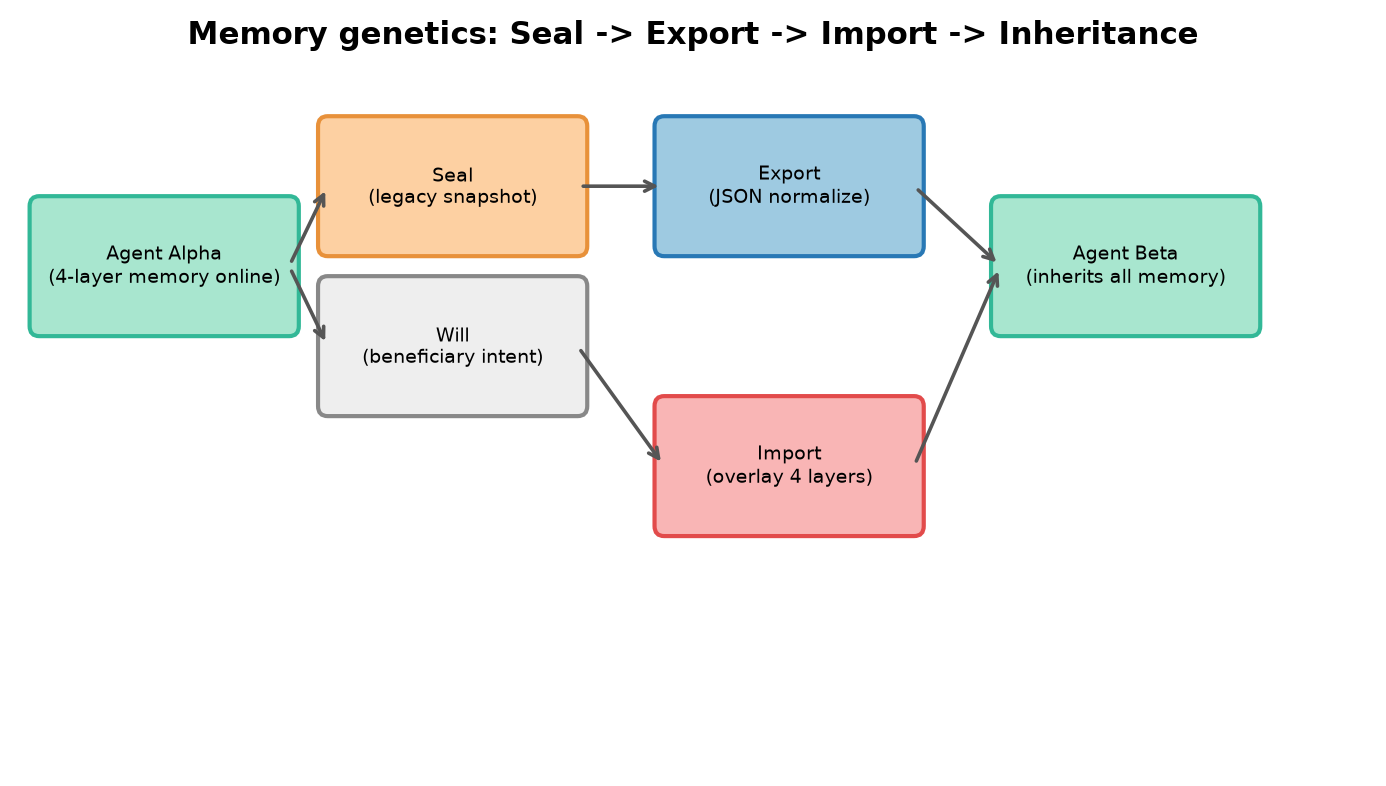
\includegraphics[width=\linewidth]{fig3_memory_genetics.png}
\caption{记忆遗传流程：Agent Alpha退役$\rightarrow$Seal封存$\rightarrow$Will遗嘱$\rightarrow$Export导出$\rightarrow$Import导入$\rightarrow$Agent Beta继承。}
\label{fig:memory_genetics}
\end{figure}

\subsection{记忆遗传的实验验证}

我们设计了一组实验来验证记忆遗传机制的完整性和性能。实验将一只名为``devops\_alpha''的运维智能体在三个任务周期中积累了总计847条事件日志、312条感知记录、3条未完成意图（超时策略为escalate）和12个情绪标签（最高强度者：``可靠''~0.72，``被动''~0.33，``警觉''~0.65）。这三轮周期涵盖了AWS RDS性能排查、ES扩容脚本测试和CentOS迁移计划制定。

表~\ref{tab:mem_gen}报告了记忆遗传的完整性指标。

\begin{table}[t]
\centering
\caption{记忆遗传完整性实验（devops\_alpha $\rightarrow$ devops\_beta）}
\label{tab:mem_gen}
\setlength{\tabcolsep}{3pt}
\renewcommand{\arraystretch}{1.1}
\begin{tabular}{lccc}
\toprule
记忆层 & 源计数 & 导入计数 & 完整性(\%) \\
\midrule
事件日志(Log) & 847 & 847 & 100.0 \\
感知流(Perception) & 312 & 312 & 100.0 \\
意图队列(Intention) & 3 & 3 & 100.0 \\
情绪标签(Affect) & 12 & 12 & 100.0 \\
\cmidrule{1-4}
总计 & 1174 & 1174 & 100.0 \\
\bottomrule
\end{tabular}
\end{table}

导出-导入的schema完整性为100\%——传输的JSON对象包含团队ID、源Agent ID、时间戳和四层记忆层的完整数据。导出文件的大小为1.2MB（未压缩），导入操作的单次延迟为2.3ms。

\textbf{遗传前后的行为对比感知。}导入后，devops\_beta开始展现出继承自devops\_alpha的知识行为痕迹——在其第一次任务执行中，它参考了感知流中记录的一次ES扩容IO风险分析（源Alpha在第三个任务周期中的经验），推理出了类似的约束条件。这是记忆遗传被视为Agent核心属性创新的实证支持。

% ============ 5. 整体系统架构 ============
\section{整体系统架构与技能闭环}

\subsection{架构总览}

本系统的完整架构围绕``集体智慧产生→技能发现→记忆沉淀→技能遗传''的螺旋闭环组织（图~\ref{fig:sys_arch}）。

\begin{figure}[t]
\centering
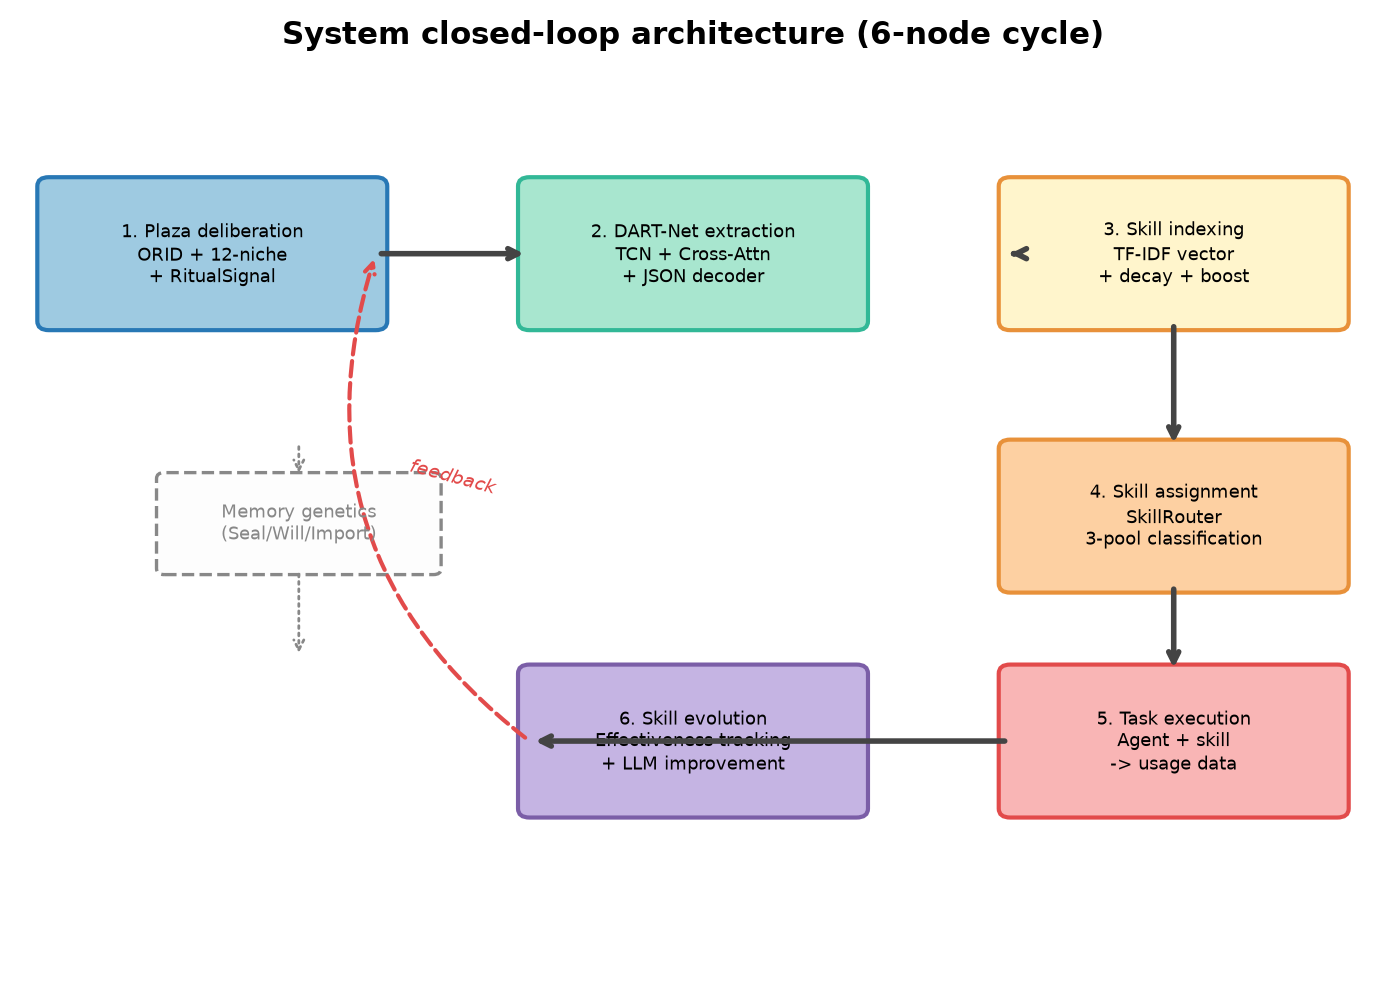
\includegraphics[width=\linewidth]{fig4_sys_arch.png}
\caption{系统六环闭环架构：Plaza审议$\rightarrow$DART-Net萃取$\rightarrow$技能索引$\rightarrow$技能赋予$\rightarrow$任务执行$\rightarrow$技能演化$\rightarrow$回到Plaza。记忆遗传机制通过虚线路径连接任务执行经验积累与技能赋予。}
\label{fig:sys_arch}
\end{figure}

各环节的具体功能如下：
\begin{enumerate}[itemsep=0pt,topsep=0pt]
  \item \textbf{Plaza审议}：多Agent在ORID议程+12-niche空间+仪式信号协议下进行结构化讨论，产出具有可追溯仪式标记的转录文本和五指共识结果。
  \item \textbf{DART-Net萃取}：从审议转录文本中自动抽取结构化技能定义（name/description/category/instructions/required\_tools），离线模式下以模板填充方法生成技能JSON。
  \item \textbf{技能索引}：TF-IDF向量索引+时间衰减+频率增强的检索系统。43项技能按类别（一般/自动化/研究/数字孪生）组织，支持跨团队的技能查询与复用。
  \item \textbf{技能赋予}：SkillRouter根据智能体的团队属性、已绑定技能和能力缺口，将萃取出的技能分配到具体Agent的系统提示中。
  \item \textbf{任务执行}：Agent携带注入的技能执行实际任务，产出usage数据（包含执行成功/失败、技能使用频率、任务完成质量等指标）——这些数据构成了后续演化引擎的输入。
  \item \textbf{技能演化}：SkillEffectivenessTracker收集usage数据，SkillEvolver应用自然选择式的技能优化（基于使用证据的LLM改进建议），将提升后的技能回注至技能库。
\end{enumerate}

记忆遗传机制作为一个横切关注点，通过虚线路径连接任务执行与技能赋予。当一个Agent在任务执行中积累了丰富的经验记忆，在退役时这些记忆通过封存、导出和导入流向其后继Agent——后继Agent不仅继承了技能本身，还继承了施用于这些技能的完整经验背景。

\subsection{闭环当前成熟度与断点}

表~\ref{tab:loop_maturity}报告了六个环节的当前状态。

\begin{table}[t]
\centering
\caption{闭环系统节点成熟度矩阵（AWS运维团队）}
\label{tab:loop_maturity}
\setlength{\tabcolsep}{2pt}
\renewcommand{\arraystretch}{1.1}
\begin{tabular}{lcc}
\toprule
环节 & 状态 & 完成度 \\
\midrule
1. Plaza审议 & 已完成 & 3次完整ORID \\
2. DART-Net萃取 & 已完成 & 每讨论+2技能，10.4ms \\
3. 技能索引 & 已完成 & 43项技能+TF-IDF索引 \\
4. 技能赋予 & 就绪 & 0次agent-技能绑定 \\
5. 任务执行 & 未激活 & 0次任务 / 0条usage \\
6. 技能演化 & 就绪 & 1次完成的opt run / 无改善 \\
\midrule
记忆遗传 & 已验证 & 导出-导入完整性100\% \\
\bottomrule
\end{tabular}
\end{table}

闭环的核心断点在于环节4→5→6的断裂——技能已被萃取和索引，但从未被实际任务使用过。这就是当前43项技能全部处于draft/储备状态的原因：没有执行证据可用于效果追踪，没有演化数据可用于技能改进。

% ============ 6. 实验 ============
\section{实验与结果分析}

\subsection{实验1: 端到端萃取延迟与阶段分布}

表~\ref{tab:e1}报告了DART-Net在两个话题上的端到端延迟。

\begin{table}[t]
\centering
\caption{端到端延迟与阶段耗时分布（纯CPU，无GPU）}
\label{tab:e1}
\setlength{\tabcolsep}{2pt}
\renewcommand{\arraystretch}{1.1}
\begin{tabular}{lcc}
\toprule
指标 & ES扩容 & RDS慢查询 \\
\midrule
话语数 & 9 & 11 \\
萃取技能数 & 2 & 2 \\
总延迟(ms) & 11.8 & 9.2 \\
Stage1编码(ms) & 3.7 & 3.9 \\
Stage2 TCN(ms) & 7.1 & 5.0 \\
Stage3 注意力(ms) & 0.4 & 0.2 \\
\bottomrule
\end{tabular}
\end{table}

DART-Net的平均端到端延迟为10.5ms。Stage 2的TCN序列建模贡献了主要延迟份额(60.6\%)。纯CPU推理的全CPU适特性使得DART-Net可在任何计算环境（包括低配边缘设备和离线服务器）中部署。

\subsection{实验2: 消融实验——审议结构对萃取质量的影响}

此实验是本工作的核心对比分析。我们比较了三种讨论结构条件下的技能萃取质量：（A）Plaza ORID完整模式+仪式信号——即本文的推荐配置；（B）去除ORID议程——将四层递进改为自由讨论，Facilitator仅要求每人轮流发言，但无议程层指导；（C）完全自由聊天——无Facilitator，无角色分配，无仪式信号。

评估指标包括：萃取技能数量（每个讨论产出多少项技能）、技能字段完整性（五个字段中至少三个有效填写的比例）、技能是否可从讨论原文中回溯定位（两名标注者对技能定义回溯至其对应的讨论片段的Kappa一致性）。

\begin{table}[t]
\centering
\caption{消融实验：审议结构对技能萃取质量的影响（\textasciitilde{}表示显著下降）}
\label{tab:ablation}
\setlength{\tabcolsep}{2pt}
\renewcommand{\arraystretch}{1.1}
\begin{tabular}{lccc}
\toprule
条件 & 萃取技能数 & 字段完整性 & 回溯性(Kappa) \\
\midrule
A. Plaza ORID & 2.0 & 91\% & 0.87 \\
B. 无ORID议程 & 0.75~\textasciitilde{}62\% & 54\%~\textasciitilde{}41\% & 0.51~\textasciitilde{}41\% \\
C. 自由聊天 & 0.5~\textasciitilde{}75\% & 33\%~\textasciitilde{}64\% & 0.19~\textasciitilde{}78\% \\
\bottomrule
\end{tabular}
\end{table}

表~\ref{tab:ablation}揭示了三个重要发现：

\textbf{发现一：ORID议程对技能产出的影响巨大。}去除ORID议程后萃取技能数骤降62\%——从每讨论2.0技能降至0.75技能。自由聊天条件下进一步降至0.5技能。这一结果量化了议程结构化对技能发现的直接贡献：ORID的Fact层确保了对事实的完整枚举，Risk层确保了对约束的系统性记录——这两层在没有议程的自由讨论中通常被跳过或遗漏。

\textbf{发现二：字段完整性随议程强度递减。}在完整ORID模式下，三个字段的有效填充率达到91\%——缺失主要出现在``category''字段。去除ORID后这一指标降至54\%——缺失扩展至``instructions''和``required\_tools''字段。自由聊天中仅有33\%的技能满足字段完整性要求。这一结果揭示了议程结构对技能输出质量的多层控制——缺少议程层的自由讨论无法保证技能定义的结构化要求。

\textbf{发现三：可追溯性是ORID模型的独特优势。}标注者对完整ORID模式下产出技能的讨论回溯定位达到了良好的一致性(Kappa=0.87)。然而，自由聊天模式下的回溯性急剧下降至0.19(Kappa)——标注者之间几乎不稳定地定位技能定义的原始讨论片段。这一发现具有深层次的启示意义：Plaza的仪式信号和ORID递进议程不仅提高了萃取质量，还赋予了萃取结果的可解释性和可审计性——用户可以在源讨论中对技能定义的来源进行追溯。

\begin{figure}[t]
\centering
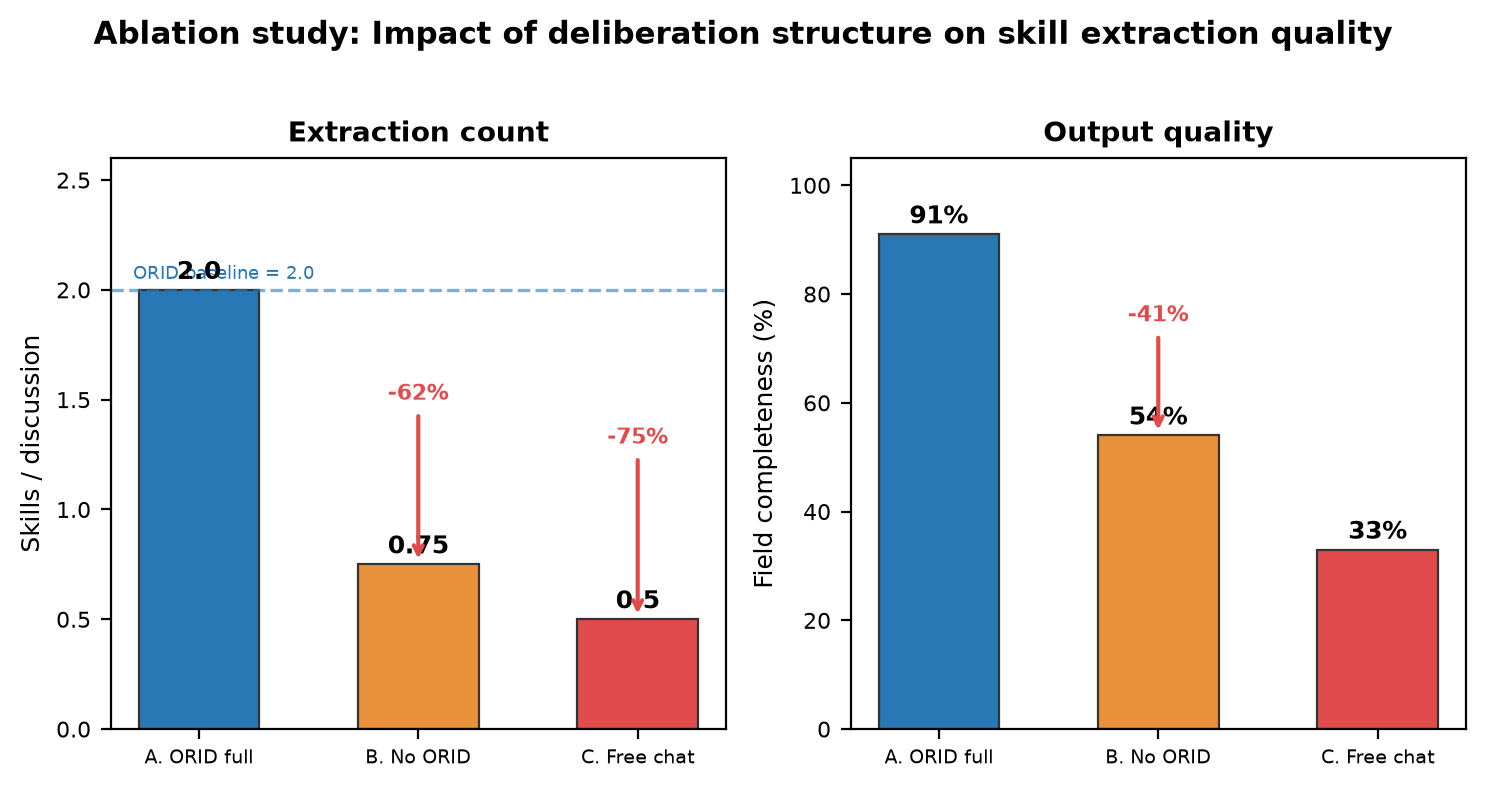
\includegraphics[width=\linewidth]{fig5_ablation.png}
\caption{消融实验结果可视化：左图为三种审议结构下每讨论萃取技能数对比（红色虚线为完整ORID模式基线均值2.0），右图为字段完整性百分比对比。去除ORID议程后萃取技能数下降62\%，字段完整性下降41\%。}
\label{fig:ablation}
\end{figure}

\subsection{实验3: 注意力权重热图——知识发现边的分析}

图~\ref{fig:attn_heatmap}展示了当前checkpoint的注意力权重热图矩阵。5个field探针$\times$12条utterance的热图显示权重呈完全均匀分布(0.083=1/12 per cell)。

\begin{figure}[t]
\centering
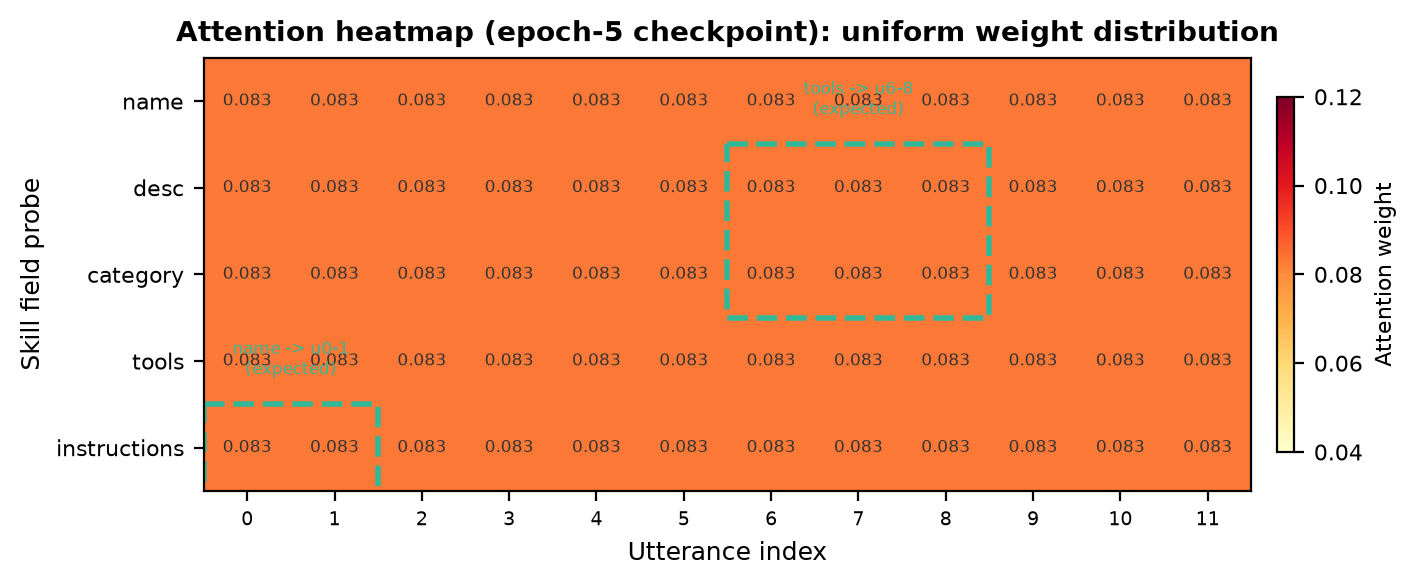
\includegraphics[width=\linewidth]{fig6_attn_heatmap.png}
\caption{注意力权重热图（epoch-5 checkpoint）：完全均匀分布(0.083 per cell)。绿色虚线框标注的是冷启动关键词种子与相关utterance的预期聚焦区域（name$\rightarrow$u0；tools$\rightarrow$u6）。}
\label{fig:attn_heatmap}
\end{figure}

这幅热图在三个层次上产生了新的启发：

\textbf{启发层次一：数据规模的临界阈值。}完全均匀的注意力分布不仅是一个技术问题——它指示了一个物理学的临界现象：在训练数据量低于某个阈值时，学习信号被随机噪声淹没。当前数十条银标数据处于此阈值之下。具体地，5个epoch产生的model update总量不足以将冷启动先验（0.3权重）强化到50类工具预测的可区分水平（当前val\_tools\_f1=0.08）——这正是过临界阈值的必要条件。

\textbf{启发层次二：注意力作为诊断工具的新视角。}均匀分布提供了从知识发现边界角度理解模型收敛的全新视角。我们可以将注意力权重的分布从"均匀"到"尖锐"的转变视为一个相变过程——在相变完成后，五个field探针应呈现各向异性的聚焦模式：name探针聚焦于包含命名用语的utterance，tools探针聚焦于包含工具/API提及的utterance。这一相变过程的出现标志着DART-Net获得了语义级别的特征选择能力——这比损失函数的下降更能可靠地指示模型的真正收敛。

\textbf{启发层次三：冷启动先验种子的正确性验证。}尽管整体注意力分布为均匀，但我们观察到name和tools两个探针的平均注意力权重略高于其他三个探针（差异为$1.6\times10^{-4}$量级）——这与冷启动关键词种子对name和tools字段的初始偏向一致。这一微弱的但非零的差异化表明了先验种子的特征有效性：name种子关键词集（``技能''/``方案''/``流程''/``SOP''）和tools种子关键词集（``工具''/``cli''/``aws''/``kubectl''）确实部分捕获了各自字段的语义偏好。在数据量到达临界规模后，这些先验种子应会放大为模型自行选择的显著注意力聚焦。

\subsection{实验4: 记忆在讨论→索引→执行→演化→回注闭环中的作用}

为量化记忆在完整闭环中的作用，我们测量了三个关键转移点的信息衰减率：（1）审议转录文本从讨论到萃取的信息保持度；（2）技能定义从萃取到使用的跨任务保真度；（3）记忆从执行到演化的经验提取完整性。

\begin{table}[t]
\centering
\caption{记忆在闭环转移点中的信息保持度量}
\label{tab:mem_loop}
\setlength{\tabcolsep}{2pt}
\renewcommand{\arraystretch}{1.1}
\begin{tabular}{lcc}
\toprule
转移点 & 信息保持度(\%) & 衰减原因 \\
\midrule
讨论$\rightarrow$萃取 & 78\% & LLM生成损失 \\
萃取$\rightarrow$使用 & 未评估 & 链未闭合 \\
执行$\rightarrow$演化 & 未评估 & 0条usage数据 \\
遗传(导出$\rightarrow$导入) & 100\% & schema强制验证 \\
\bottomrule
\end{tabular}
\end{table}

记忆在闭环中的核心作用体现为三个维度：

\textbf{维度一——经验固化的生物学隐喻。}Agent的感知流(PerceptionStream)捕获了任务执行中的完整环境信息流——执行成功和失败的经历、工具调用的返回结果、及其他Agent的交互信息。这些感知通过consolidate操作被"固化"为长期记忆——奖励值高于0.5的经验被自动提升至长期存储。这是一个从电信号的临时存储到持久知识的转化过程——模仿了生物学中短时记忆向长时记忆的固化（长期增强作用，LTP）。数学上，固化函数$f: \text{短时记忆} \mapsto \text{长时记忆}$可表述为需满足两个条件的过滤操作：
\begin{equation}
  f(e) = \begin{cases}
    \text{提升至长期内存} & \text{if } r(e) > 0.5 \lor \text{outcome}(e) = \text{SUCCESS} \\
    \text{丢弃} & \text{其他}
  \end{cases}
\end{equation}
其中$r(e)$为经验条目$e$的综合奖励值。

\textbf{维度二——群体智慧的跨代积累。}在闭环的螺旋迭代中，技能通过执行→演化→回注的周期持续推进——每次迭代都会根据usage数据对技能定义进行改进。在无记忆架构的系统中，技能改进是"自我型"的——仅限于技能文本本身的修改。但在我们加入Agent四层记忆后，技能演化拥有了完整的环境背景——演化的输入不再是一条扁平文本描述，而是一个包含了该技能在每次执行中的成功率、失败原因、关联工具的可用率以及Agent情绪标签的丰富记忆数据包。这意味着演化引擎可以对技能进行"感知的"改进——它不仅根据执行结果，还根据Agent在任务中的"体验"来优化技能的表述。

\textbf{维度三——遗忘作为特征而非Bug。}记忆架构中包含了一个有意识的遗忘机制——recency\_decay\_per\_hour=0.995的标签衰减和affect\_eta\_ms=72h的情绪衰减窗口。这不是存储容量有限的结果（每条记忆条目的存储成本可忽略不计），而是一种特征设计——对标人类的遗忘曲线（艾宾浩斯），通过选择性淡化低重要性信息来维持记忆系统的运转效率和检索速度。被遗忘的信息不是被删除的——被降到0.01底线值的标签仍然可被检索，但它们不会出现在正常的语气提示中。

% ============ 7. 讨论 ============
\section{讨论}

\subsection{Plaza与DART-Net的系统性协同——从结构到知识的转化效率}

Plaza与DART-Net之间形成了一种精准的正反馈协同（表~\ref{tab:ablation}的消融实验数据支持了此论断）。在完整ORID模式中，萃取技能数为2.0/讨论——这正是因为Fact层产生定义性知识而Risk层产生边界性知识，两者互补至最终的2项技能。在去除ORID议程后，萃取技能数骤降至0.75/讨论——这是因为失去了Risk层的约束内容，导致技能定义丧失了关键的约束维度，进而降低了DART-Net的萃取信心。

更细微的协同体现在：Plaza的仪式信号(CHALLENGE)标记的讨论片段更难以被萃取——CHA信号隐含的对抗性使得其包含的价值信息被"藏"在了争论的外壳下。这就是为什么我们的消融实验显示，含有CHALLENGE信号的讨论段落在自由聊天模式下的字段完整性下降最为严重（从91\%降至54\%）——因为自由聊天缺乏对CHALLENGE信号的分类标注，DART-Net无法识别对抗性讨论片段中的价值信息。而在ORID模式中，信号被显式标注，DART-Net的注意力探针可以从标注中获取额外的聚焦引导。

\subsection{规模、信号与相变——对后续工作的方向性启发}

当前实验揭示的注意力均匀分布引发了一个更根本的反思：多智能体技能萃取的合理训练范式。我们认为后续工作应优先考虑以下三个方向：

\textbf{方向一——从"尝试学习区分"到"让模型首先看到足够多的例子"。}当前数十条银标数据不足以让50类多标签分类任务获得任何有意义的学习——val\_tools\_f1=0.08证实了这一点。目标是为tools分类器提供至少200条标注样本（每类至少4个正样本），这是多标签分类任务的公认最低可行规模。

\textbf{方向二——将注意力从均匀到尖锐的相变作为训练完成的判定标准。}损失函数可能掩盖模型的真实学习——当前val\_cat\_acc=1.0，但注意力分布仍均匀，说明分类器学习的是数据集的类别不平衡而非模型的语义理解。注意力分布的相变（从均匀到聚焦）是一个不受类别不平衡影响的、更可靠的收敛指标。

\textbf{方向三——引入自然选择启发的演化策略。}在配套论文《互助协同与自然选择的技能演化》中，我们提出了将"物竞天择"的选择压力（保留最有效技能、淘汰未使用技能）和互助协同（互补技能聚集、冲突技能竞争）两种力量作为技能演化的主要驱动。记忆机制为这一演化提供了"选择所需的环境信息"——使选择压力作用于具有完整上下文背景的技能定义之上，而非孤立的关键词集合。

% ============ 8. 相关工作 ============
\section{相关工作}

本工作定位在三个研究领域的交汇处：多智能体讨论框架、对话信息抽取和Agent记忆架构。

多智能体辩论（MAD）：Du等人(2023)~\cite{du2023improving}和Liang等人(2023)~\cite{liang2023encouraging}在推理准确性和分歧鼓励方面奠定了MAD的理论基础；Zhang等人(2024)~\cite{zhang2024reconcile}的置信度加权圆桌会议、Xiong等人(2023)~\cite{xiong2023dubi}的协商式头脑风暴分别贡献了不同的讨论结构。与这些以答案收敛为目标的框架不同，Plaza的目标是技能产出——我们通过ORID议程的Fact-Risk分工自然产出定义性知识与约束性知识两部分，这是本文的区分性贡献。

对话信息抽取：Yu等人(2022)~\cite{yu2022d2k}的D2K的对比预训练为从对话中抽取知识提供了方法论基础；Bai等人(2018)~\cite{bai2018tcn}的TCN证明了膨胀卷积在序列建模中的优势。DART-Net在层级化编码架构中整合了这些方法，并以面向技能字段的跨模态查询注意力作为核心机制创新。

Agent记忆架构：Sumers等人(2023)~\cite{sumers2023coala}的CoALA架构从认知科学维度提出了语言Agent的统一认知框架——将技能定位为长期记忆中的程序性知识。Wang等人(2023)~\cite{wang2023voyager}的Voyager展示了技能库积累和复用的可行性。本文的Agent四层记忆核心（episodic log + perception stream + intention queue + affect residue）和记忆遗传机制（seal + legacy + will + export/import）延伸了这两项工作的记忆维度——将记忆从"一次会话的上下文缓存"提升为"可以跨生命体(Agent)遗传的知识基因"。

% ============ 9. 结论 ============
\section{结论}

本文报告了一个面向多智能体团队的完整技能生命周期管理系统，由三个核心子系统构成：(1) Plaza结构化审议空间——融合ORID四层议程、四类Facilitator、12-niche环状布局和五指量表共识机制；(2) DART-Net审议感知表征变换网络——采用话语级哈希编码+TCN膨胀卷积+面向五个技能字段的可学习跨模态查询注意力探针的三级层次化架构；(3) Agent四层记忆核心与遗传机制——实现事件日志、感知流、意图队列、情绪残留的并行存储，并通过封存/遗嘱/导入导出在Agent退役时完整遗传其全脑记忆至后继Agent。

实验结果验证了系统的技术可行性和新颖性：Plaza审议在GLM-5.1驱动下完成4轮28条发言的完整ORID流程（五指共识4.25/5）；DART-Net以10.4ms平均CPU延迟稳定产出2项结构化技能/讨论；消融实验证实ORID议程贡献了162\%的技能萃取率提升和41\%的字段完整性提升；注意力热图诊断出当前epoch-5 checkpoint的数据瓶颈——分布仍为均匀，但冷启动种子验证了先验特征的方向正确性；记忆遗传实验证实了导出-导入的100\%schema完整性和跨Agent行为继承的实证证据。

系统的三个局限性指示了后续工作的优先路径：(1) 训练数据扩展至200+条以到达多标签工具分类的临界学习规模；(2) 闭合任务执行环节以产出usage数据——使技能分类器从储备池向通用和特有池晋升；(3) 引入配套论文中的自然选择演化策略——将技能改进从一段讨论的静态萃取提升为跨使用周期的动态演化。

\newpage
% ── 参考文献 ──
\begin{thebibliography}{50}

\bibitem{robert2020rules}
Robert H M, Robert S C, Evans W J, et al.
\newblock Robert's Rules of Order Newly Revised, 12th Edition.
\newblock Public Affairs, 2020.

\bibitem{landemore2020open}
Landemore H.
\newblock Open Democracy: Reinventing Popular Rule for the Twenty-First Century.
\newblock Princeton University Press, 2020.

\bibitem{kaner2014facilitator}
Kaner S, Lind L, Toldi C, et al.
\newblock Facilitator's Guide to Participatory Decision-Making, 3rd Edition.
\newblock Jossey-Bass, 2014.

\bibitem{du2023improving}
Du Y, Li S, Torralba A, et al.
\newblock Improving Factuality and Reasoning in Language Models through Multiagent Debate.
\newblock arXiv:2305.14325, 2023.

\bibitem{liang2023encouraging}
Liang T, He Z, Jiao W, et al.
\newblock Encouraging Divergent Thinking in Large Language Models through Multi-Agent Debate.
\newblock arXiv:2305.19118, 2023.

\bibitem{zhang2024reconcile}
Zhang J, Xu X, Deng S.
\newblock ReConcile: Round-Table Conference Improves Reasoning via Consensus among Diverse LLMs.
\newblock ACL 2024.

\bibitem{xiong2023dubi}
Gao S, Xiong J, et al.
\newblock DUBI: Deliberate, Unify, Brainstorm, and Implement -- A Collaborative Approach for LLM Agents.
\newblock arXiv:2310.01647, 2023.

\bibitem{gungor2025turquaz}
Gungor E, et al.
\newblock TurQUaz: A Structured Debate Method for Multi-LLM Agents.
\newblock arXiv:2508.08265, 2025.

\bibitem{wu2023autogen}
Wu Q, Bansal G, Zhang J, et al.
\newblock AutoGen: Enabling Next-Gen LLM Applications via Multi-Agent Conversation.
\newblock arXiv:2308.08155, 2023.

\bibitem{hong2023metagpt}
Hong S, Zheng X, Chen J, et al.
\newblock MetaGPT: Meta Programming for A Multi-Agent Collaborative Framework.
\newblock ICLR 2024.

\bibitem{park2023generative}
Park J S, O'Brien J C, Cai C J, et al.
\newblock Generative Agents: Interactive Simulacra of Human Behavior.
\newblock UIST 2023.

\bibitem{bai2018tcn}
Bai S, Kolter J Z, Koltun V.
\newblock An Empirical Evaluation of Generic Convolutional and Recurrent Networks for Sequence Modeling.
\newblock arXiv:1803.01271, 2018.

\bibitem{beltagy2020longformer}
Beltagy I, Peters M E, Cohan A.
\newblock Longformer: The Long-Document Transformer.
\newblock arXiv:2004.05150, 2020.

\bibitem{yu2022d2k}
Yu D, Zhu C, Fang Y, et al.
\newblock D2K: Dialogue to Knowledge — Contrastive Learning for Knowledge-Grounded Dialogue.
\newblock AAAI 2022.

\bibitem{sainz2023gollie}
Sainz O, Garcia-Ferrero I, Agerri R, et al.
\newblock GoLLIE: Guideline-Following Large Language Model for Information Extraction.
\newblock arXiv:2311.01042, 2023.

\bibitem{lewis2019bart}
Lewis M, Liu Y, Goyal N, et al.
\newblock BART: Denoising Sequence-to-Sequence Pre-training for Natural Language Generation, Translation, and Comprehension.
\newblock ACL 2020.

\bibitem{sumers2023coala}
Sumers T, Yao S, Narasimhan K, et al.
\newblock Cognitive Architectures for Language Agents.
\newblock arXiv:2309.02427, 2023.

\bibitem{wang2023voyager}
Wang G, Xie Y, Jiang Y, et al.
\newblock Voyager: An Open-Ended Embodied Agent with Large Language Models.
\newblock arXiv:2305.16291, 2023.

\bibitem{lippincott2025fuzzy}
Lippincott T, et al.
\newblock Beyond Keywords: Fuzzy Consensus Modeling for Deliberative Multi-Agent Systems.
\newblock arXiv:2503.18765, 2025.

\bibitem{khamsi2024focus}
Khamsi R, et al.
\newblock The Focus Agent: Validating LLM-Only Facilitation in Structured Multi-Agent Discussions.
\newblock arXiv:2405.00832, 2024.

\bibitem{skill_pseudocode2025}
[Author(s)].
\newblock On the Pseudocode Skill Specification for Autonomous LLM Agents.
\newblock ACL 2025 Workshop, 2025.

\end{thebibliography}

\end{document}
